% Options for packages loaded elsewhere
\PassOptionsToPackage{unicode}{hyperref}
\PassOptionsToPackage{hyphens}{url}
\documentclass[
  ignorenonframetext,
]{beamer}
\newif\ifbibliography
\usepackage{pgfpages}
\setbeamertemplate{caption}[numbered]
\setbeamertemplate{caption label separator}{: }
\setbeamercolor{caption name}{fg=normal text.fg}
\beamertemplatenavigationsymbolsempty
% remove section numbering
\setbeamertemplate{part page}{
  \centering
  \begin{beamercolorbox}[sep=16pt,center]{part title}
    \usebeamerfont{part title}\insertpart\par
  \end{beamercolorbox}
}
\setbeamertemplate{section page}{
  \centering
  \begin{beamercolorbox}[sep=12pt,center]{section title}
    \usebeamerfont{section title}\insertsection\par
  \end{beamercolorbox}
}
\setbeamertemplate{subsection page}{
  \centering
  \begin{beamercolorbox}[sep=8pt,center]{subsection title}
    \usebeamerfont{subsection title}\insertsubsection\par
  \end{beamercolorbox}
}
% Prevent slide breaks in the middle of a paragraph
\widowpenalties 1 10000
\raggedbottom
\AtBeginPart{
  \frame{\partpage}
}
\AtBeginSection{
  \ifbibliography
  \else
    \frame{\sectionpage}
  \fi
}
\AtBeginSubsection{
  \frame{\subsectionpage}
}
\usepackage{iftex}
\ifPDFTeX
  \usepackage[T1]{fontenc}
  \usepackage[utf8]{inputenc}
  \usepackage{textcomp} % provide euro and other symbols
\else % if luatex or xetex
  \usepackage{unicode-math} % this also loads fontspec
  \defaultfontfeatures{Scale=MatchLowercase}
  \defaultfontfeatures[\rmfamily]{Ligatures=TeX,Scale=1}
\fi
\usepackage{lmodern}
\ifPDFTeX\else
  % xetex/luatex font selection
\fi
% Use upquote if available, for straight quotes in verbatim environments
\IfFileExists{upquote.sty}{\usepackage{upquote}}{}
\IfFileExists{microtype.sty}{% use microtype if available
  \usepackage[]{microtype}
  \UseMicrotypeSet[protrusion]{basicmath} % disable protrusion for tt fonts
}{}
\makeatletter
\@ifundefined{KOMAClassName}{% if non-KOMA class
  \IfFileExists{parskip.sty}{%
    \usepackage{parskip}
  }{% else
    \setlength{\parindent}{0pt}
    \setlength{\parskip}{6pt plus 2pt minus 1pt}}
}{% if KOMA class
  \KOMAoptions{parskip=half}}
\makeatother
\usepackage{color}
\usepackage{fancyvrb}
\newcommand{\VerbBar}{|}
\newcommand{\VERB}{\Verb[commandchars=\\\{\}]}
\DefineVerbatimEnvironment{Highlighting}{Verbatim}{commandchars=\\\{\}}
% Add ',fontsize=\small' for more characters per line
\usepackage{framed}
\definecolor{shadecolor}{RGB}{248,248,248}
\newenvironment{Shaded}{\begin{snugshade}}{\end{snugshade}}
\newcommand{\AlertTok}[1]{\textcolor[rgb]{0.94,0.16,0.16}{#1}}
\newcommand{\AnnotationTok}[1]{\textcolor[rgb]{0.56,0.35,0.01}{\textbf{\textit{#1}}}}
\newcommand{\AttributeTok}[1]{\textcolor[rgb]{0.13,0.29,0.53}{#1}}
\newcommand{\BaseNTok}[1]{\textcolor[rgb]{0.00,0.00,0.81}{#1}}
\newcommand{\BuiltInTok}[1]{#1}
\newcommand{\CharTok}[1]{\textcolor[rgb]{0.31,0.60,0.02}{#1}}
\newcommand{\CommentTok}[1]{\textcolor[rgb]{0.56,0.35,0.01}{\textit{#1}}}
\newcommand{\CommentVarTok}[1]{\textcolor[rgb]{0.56,0.35,0.01}{\textbf{\textit{#1}}}}
\newcommand{\ConstantTok}[1]{\textcolor[rgb]{0.56,0.35,0.01}{#1}}
\newcommand{\ControlFlowTok}[1]{\textcolor[rgb]{0.13,0.29,0.53}{\textbf{#1}}}
\newcommand{\DataTypeTok}[1]{\textcolor[rgb]{0.13,0.29,0.53}{#1}}
\newcommand{\DecValTok}[1]{\textcolor[rgb]{0.00,0.00,0.81}{#1}}
\newcommand{\DocumentationTok}[1]{\textcolor[rgb]{0.56,0.35,0.01}{\textbf{\textit{#1}}}}
\newcommand{\ErrorTok}[1]{\textcolor[rgb]{0.64,0.00,0.00}{\textbf{#1}}}
\newcommand{\ExtensionTok}[1]{#1}
\newcommand{\FloatTok}[1]{\textcolor[rgb]{0.00,0.00,0.81}{#1}}
\newcommand{\FunctionTok}[1]{\textcolor[rgb]{0.13,0.29,0.53}{\textbf{#1}}}
\newcommand{\ImportTok}[1]{#1}
\newcommand{\InformationTok}[1]{\textcolor[rgb]{0.56,0.35,0.01}{\textbf{\textit{#1}}}}
\newcommand{\KeywordTok}[1]{\textcolor[rgb]{0.13,0.29,0.53}{\textbf{#1}}}
\newcommand{\NormalTok}[1]{#1}
\newcommand{\OperatorTok}[1]{\textcolor[rgb]{0.81,0.36,0.00}{\textbf{#1}}}
\newcommand{\OtherTok}[1]{\textcolor[rgb]{0.56,0.35,0.01}{#1}}
\newcommand{\PreprocessorTok}[1]{\textcolor[rgb]{0.56,0.35,0.01}{\textit{#1}}}
\newcommand{\RegionMarkerTok}[1]{#1}
\newcommand{\SpecialCharTok}[1]{\textcolor[rgb]{0.81,0.36,0.00}{\textbf{#1}}}
\newcommand{\SpecialStringTok}[1]{\textcolor[rgb]{0.31,0.60,0.02}{#1}}
\newcommand{\StringTok}[1]{\textcolor[rgb]{0.31,0.60,0.02}{#1}}
\newcommand{\VariableTok}[1]{\textcolor[rgb]{0.00,0.00,0.00}{#1}}
\newcommand{\VerbatimStringTok}[1]{\textcolor[rgb]{0.31,0.60,0.02}{#1}}
\newcommand{\WarningTok}[1]{\textcolor[rgb]{0.56,0.35,0.01}{\textbf{\textit{#1}}}}
\usepackage{longtable,booktabs,array}
\usepackage{calc} % for calculating minipage widths
\usepackage{caption}
% Make caption package work with longtable
\makeatletter
\def\fnum@table{\tablename~\thetable}
\makeatother
\usepackage{graphicx}
\makeatletter
\newsavebox\pandoc@box
\newcommand*\pandocbounded[1]{% scales image to fit in text height/width
  \sbox\pandoc@box{#1}%
  \Gscale@div\@tempa{\textheight}{\dimexpr\ht\pandoc@box+\dp\pandoc@box\relax}%
  \Gscale@div\@tempb{\linewidth}{\wd\pandoc@box}%
  \ifdim\@tempb\p@<\@tempa\p@\let\@tempa\@tempb\fi% select the smaller of both
  \ifdim\@tempa\p@<\p@\scalebox{\@tempa}{\usebox\pandoc@box}%
  \else\usebox{\pandoc@box}%
  \fi%
}
% Set default figure placement to htbp
\def\fps@figure{htbp}
\makeatother
\setlength{\emergencystretch}{3em} % prevent overfull lines
\providecommand{\tightlist}{%
  \setlength{\itemsep}{0pt}\setlength{\parskip}{0pt}}
\usepackage{bookmark}
\IfFileExists{xurl.sty}{\usepackage{xurl}}{} % add URL line breaks if available
\urlstyle{same}
\hypersetup{
  pdftitle={Lab 5},
  pdfauthor={Ray Caraher},
  hidelinks,
  pdfcreator={LaTeX via pandoc}}

\title{Lab 5}
\author{Ray Caraher}
\date{2025-04-21}

\begin{document}
\frame{\titlepage}

\section{Setup}\label{setup}

\begin{frame}[fragile]{Setting up our script}
\phantomsection\label{setting-up-our-script}
Before we get into any real coding, let's make sure that the preamble
for our code looks good. Here is how I set it up:

\tiny

\begin{Shaded}
\begin{Highlighting}[]
\DocumentationTok{\#\# Load packages}
\FunctionTok{library}\NormalTok{(haven)}
\FunctionTok{library}\NormalTok{(tidyverse)}
\DocumentationTok{\#\# Set options}

\FunctionTok{options}\NormalTok{(}\AttributeTok{scipen =} \DecValTok{999}\NormalTok{)}

\DocumentationTok{\#\# Clear environment}

\FunctionTok{rm}\NormalTok{(}\AttributeTok{list =} \FunctionTok{ls}\NormalTok{())}

\DocumentationTok{\#\# Set directories}

\NormalTok{base\_directory }\OtherTok{\textless{}{-}} \StringTok{\textquotesingle{}/Users/rcaraher/Library/CloudStorage/OneDrive{-}UniversityofMassachusetts/Academic/Teaching/ECON 755/Problem Sets\textquotesingle{}}
\NormalTok{data\_directory }\OtherTok{\textless{}{-}} \FunctionTok{file.path}\NormalTok{(base\_directory, }\StringTok{\textquotesingle{}Data\textquotesingle{}}\NormalTok{)}
\NormalTok{results\_directory }\OtherTok{\textless{}{-}} \FunctionTok{file.path}\NormalTok{(base\_directory, }\StringTok{\textquotesingle{}Results\textquotesingle{}}\NormalTok{)}
\end{Highlighting}
\end{Shaded}
\end{frame}

\section{Machine Learning in R}\label{machine-learning-in-r}

\begin{frame}{Intro to Machine Learning}
\phantomsection\label{intro-to-machine-learning}
In this section fo the class, forget about \textbf{causality} (e.g, does
the minimum wage cause unemployment?)

For now, focus on \textbf{prediction} (e.g., who is more likely to be a
minimum wage worker?)
\end{frame}

\begin{frame}{What's the Goal?}
\phantomsection\label{whats-the-goal}
\begin{itemize}
\tightlist
\item
  \textbf{Causal inference}

  \begin{itemize}
  \tightlist
  \item
    Estimate the effect of a policy/treatment (e.g.~Y caused by D)\\
  \item
    Answer ``What if\ldots?'' questions\\
  \end{itemize}
\item
  \textbf{Prediction}

  \begin{itemize}
  \tightlist
  \item
    Forecast Y given X\\
  \item
    Answer ``How well can I guess Y?''
  \end{itemize}
\end{itemize}
\end{frame}

\begin{frame}{Identification vs.~Generalization}
\phantomsection\label{identification-vs.-generalization}
\begin{longtable}[]{@{}
  >{\raggedright\arraybackslash}p{(\linewidth - 4\tabcolsep) * \real{0.2683}}
  >{\raggedright\arraybackslash}p{(\linewidth - 4\tabcolsep) * \real{0.3780}}
  >{\raggedright\arraybackslash}p{(\linewidth - 4\tabcolsep) * \real{0.3537}}@{}}
\toprule\noalign{}
\begin{minipage}[b]{\linewidth}\raggedright
Aspect
\end{minipage} & \begin{minipage}[b]{\linewidth}\raggedright
Causal Inference
\end{minipage} & \begin{minipage}[b]{\linewidth}\raggedright
Prediction
\end{minipage} \\
\midrule\noalign{}
\endhead
Core focus & Identification of treatment effect & Minimizing prediction
error \\
Required assumptions & Validity of research design & None;
``data-driven'' process \\
Evaluation metric & standard errors & ``fit'' statistics \\
``Cross‐validation'' & Placebo tests, sensitivity analysis & K‑fold CV,
hold‑out test set \\
\bottomrule\noalign{}
\end{longtable}
\end{frame}

\begin{frame}{Combining Machine Learning and Causal Inference}
\phantomsection\label{combining-machine-learning-and-causal-inference}
Despite very different worlds, predictive tools from machine learning
can be used in lots of creative ways for causal inference!
\end{frame}

\begin{frame}{From a Causal Question to a Prediction Problem}
\phantomsection\label{from-a-causal-question-to-a-prediction-problem}
Recall rational for looking at the effect of minimum wage laws on
teenagers:

\begin{itemize}
\tightlist
\item
  They are most likely to be directly affected by the policy (i.e., the
  sharpest ``bite''), so we should focus on them to understand the
  effect of these policies
\end{itemize}

But the reality of \textbf{who} is likely to be a minimum wage worker is
likely more complex than just age

\begin{itemize}
\tightlist
\item
  race, education, etc. are also likely to be important!
\item
  Using a \emph{single predictor} (age) may understate the likelihood
  someone is part of the group which may be most affected by the policy
  change
\end{itemize}

Now, instead of a causal problem, we have (for a minute) a
\textbf{prediction problem}
\end{frame}

\begin{frame}{Problem Set Question}
\phantomsection\label{problem-set-question}
We want to predict \textbf{who} is most likely to be a minimum wage
worker so we can study the effect of minimum wage policies \emph{on that
group}

We will use a basic machine learning exercise to do so
\end{frame}

\section{Overview of Machine
Learning}\label{overview-of-machine-learning}

\begin{frame}{1. Problem Definition}
\phantomsection\label{problem-definition}
\begin{itemize}
\tightlist
\item
  \textbf{Objective}: What are we trying to predict or learn?\\
\item
  \textbf{Type of task}:

  \begin{itemize}
  \tightlist
  \item
    Supervised (regression, classification: we have a ``Y'' variable)\\
  \item
    Unsupervised (clustering, dimensionality reduction: no ``Y''
    variable; looking for patterns in the data)
  \end{itemize}
\end{itemize}
\end{frame}

\begin{frame}{2. Data Collection \& Preparation}
\phantomsection\label{data-collection-preparation}
\begin{itemize}
\tightlist
\item
  \textbf{Inspect \& clean}:

  \begin{itemize}
  \tightlist
  \item
    Handle missing values, outliers\\
  \item
    Correct typos, standardize formats\\
  \end{itemize}
\item
  \textbf{Split} into training/test sets (e.g.~50/50, 80/20, etc.)
\end{itemize}
\end{frame}

\begin{frame}{3. Feature (Variables) Engineering}
\phantomsection\label{feature-variables-engineering}
\begin{itemize}
\tightlist
\item
  \textbf{Transform raw inputs} into features:

  \begin{itemize}
  \tightlist
  \item
    Scaling/normalization\\
  \item
    Interaction terms, polynomial features\\
  \end{itemize}
\item
  \textbf{Dimensionality reduction} (if needed):

  \begin{itemize}
  \tightlist
  \item
    PCA, feature selection\\
  \end{itemize}
\item
  \textbf{Domain knowledge}:

  \begin{itemize}
  \tightlist
  \item
    Craft features informed by theory or context
  \end{itemize}
\end{itemize}
\end{frame}

\begin{frame}{4. Model Selection \& Training}
\phantomsection\label{model-selection-training}
\begin{itemize}
\tightlist
\item
  \textbf{Choose candidate algorithms}

  \begin{itemize}
  \tightlist
  \item
    Linear models (logistic regression, LASSO), tree‑based (RF, GBM),
    nueral nets
  \end{itemize}
\item
  \textbf{Hyperparameter tuning}

  \begin{itemize}
  \tightlist
  \item
    Cross validation to find optimal hyperparameters
  \end{itemize}
\item
  \textbf{Train models} on training set
\end{itemize}
\end{frame}

\begin{frame}{5. Evaluation \& Validation}
\phantomsection\label{evaluation-validation}
\begin{itemize}
\tightlist
\item
  \textbf{Assess performance} on test sets

  \begin{itemize}
  \tightlist
  \item
    Regression: RMSE, R-squared
  \item
    Classification: accuracy, AUC, precision/recall\\
  \end{itemize}
\item
  \textbf{Diagnostics}

  \begin{itemize}
  \tightlist
  \item
    Learning curves, bias--variance trade‑off
  \end{itemize}
\item
  \textbf{Robustness checks}

  \begin{itemize}
  \tightlist
  \item
    Sensitivity to hyperparameters, data subsets
  \end{itemize}
\end{itemize}
\end{frame}

\begin{frame}{6. Deployment}
\phantomsection\label{deployment}
\begin{itemize}
\tightlist
\item
  \textbf{Deploy model} to make predictions on ``final'' data
\end{itemize}
\end{frame}

\begin{frame}{Pipline for Our Problem}
\phantomsection\label{pipline-for-our-problem}
We want to:

\begin{enumerate}
\tightlist
\item
  \textbf{Get micro-data} from the CPS MORG data (contains
  individual-level demographic info)
\item
  \textbf{Pre-process} our ``features'' (i.e., variables) and data
\item
  \textbf{Split} our data into training/test sets
\item
  \textbf{Train} our model using a ML method on the training data
  (gradient boosting)
\item
  \textbf{Evaluate} our model using the test data (precision-recall
  curve)
\item
  \textbf{Deploy} our model on the full data
\item
  \textbf{Calculate} employment and wage rates for likely minimum wage
  workers
\item
  \textbf{Estimate} the effect of CA's MW increase on the
  employment/wage rates of those workers
\end{enumerate}
\end{frame}

\begin{frame}[fragile]{MORG data}
\phantomsection\label{morg-data}
Let's read in the MORG data and take a look at it

\scriptsize

\begin{Shaded}
\begin{Highlighting}[]
\NormalTok{morg }\OtherTok{\textless{}{-}} \FunctionTok{read\_dta}\NormalTok{(}\FunctionTok{file.path}\NormalTok{(data\_directory, }\StringTok{"CPSmorg\_1979\_1990\_small.dta"}\NormalTok{))}

\FunctionTok{glimpse}\NormalTok{(morg)}
\end{Highlighting}
\end{Shaded}

\begin{verbatim}
## Rows: 4,126,876
## Columns: 16
## $ month       <dbl+lbl>  4,  4, 10,  9,  8,  8,  8,  2, 12,  4,  8,  6,  5, 11~
## $ hhid        <chr> "301093021702", "808342401006", "808012816108", "732093299~
## $ state       <dbl+lbl> NA, NA, NA, NA, NA, NA, NA, NA, NA, NA, NA, NA, NA, NA~
## $ age         <dbl> 72, 57, 61, 33, 34, 32, 31, 36, 37, 39, 28, 64, 30, 27, 21~
## $ race        <dbl+lbl> 1, 1, 1, 1, 1, 1, 1, 1, 1, 1, 1, 1, 1, 1, 1, 1, 1, 1, ~
## $ sex         <dbl+lbl> 0, 0, 0, 0, 1, 1, 1, 0, 0, 1, 1, 0, 1, 0, 1, 0, 0, 0, ~
## $ esr         <dbl+lbl>  4,  4,  4,  1,  3,  2,  1, NA,  1,  1, NA,  4,  1,  4~
## $ earnhre     <dbl> NA, NA, NA, NA, NA, 420, 375, 395, 1111, NA, NA, NA, NA, N~
## $ year        <dbl> 1981, 1980, 1981, 1987, 1980, 1980, 1981, 1989, 1985, 1980~
## $ statenum    <dbl+lbl> 23, 23, 23, 23, 23, 23, 23, 23, 23, 23, 23, 23, 23, 23~
## $ cpi         <dbl> 38.79457, 35.28579, 40.29428, 49.91511, 36.38936, 36.38936~
## $ hispanic    <dbl> 0, 0, 0, 0, 0, 0, 0, 0, 0, 0, 0, 0, 0, 0, 0, 0, 0, 0, 0, 0~
## $ dmarried    <dbl> 1, 1, 1, 0, 0, 0, 1, 0, 1, 1, 1, 1, 1, 1, 0, 0, 1, 0, 1, 1~
## $ ruralstatus <dbl> 2, 2, 2, 2, 2, 2, 2, 2, 1, 2, 2, 1, 2, 2, 1, 2, 1, 1, 2, 2~
## $ veteran     <dbl> 0, 0, 0, 0, 0, 1, 1, 0, 0, 0, 0, 0, 1, 0, 0, 0, 0, 0, 0, 0~
## $ educcat     <dbl> 1, 3, 1, 4, 2, 2, 2, 3, 4, 2, 4, 2, 2, 2, 2, 2, 2, 2, 2, 3~
\end{verbatim}
\end{frame}

\begin{frame}[fragile]{Feature engineering}
\phantomsection\label{feature-engineering}
Let's now process our data to get it ready for our ML technique

\tiny

\begin{Shaded}
\begin{Highlighting}[]
\DocumentationTok{\#\# Define minimum wage worker}

\NormalTok{morg }\OtherTok{\textless{}{-}}\NormalTok{ morg }\SpecialCharTok{|\textgreater{}}
  \FunctionTok{mutate}\NormalTok{(}\AttributeTok{mw =} \FunctionTok{case\_when}\NormalTok{(earnhre }\SpecialCharTok{\textgreater{}} \DecValTok{100} \SpecialCharTok{\&}\NormalTok{ earnhre }\SpecialCharTok{\textless{}} \DecValTok{335} \SpecialCharTok{\textasciitilde{}} \DecValTok{1}\NormalTok{,}
                        \FunctionTok{is.na}\NormalTok{(earnhre) }\SpecialCharTok{\textasciitilde{}} \ConstantTok{NA\_real\_}\NormalTok{,}
                        \ConstantTok{TRUE} \SpecialCharTok{\textasciitilde{}} \DecValTok{0}\NormalTok{))}

\FunctionTok{count}\NormalTok{(morg, mw)}
\end{Highlighting}
\end{Shaded}

\begin{verbatim}
## # A tibble: 3 x 2
##      mw       n
##   <dbl>   <int>
## 1     0 1190027
## 2     1   90077
## 3    NA 2846772
\end{verbatim}
\end{frame}

\begin{frame}[fragile]
\tiny

\begin{Shaded}
\begin{Highlighting}[]
\DocumentationTok{\#\#\# Convert to factors}

\NormalTok{morg }\OtherTok{\textless{}{-}}\NormalTok{ morg }\SpecialCharTok{|\textgreater{}}
  \FunctionTok{mutate}\NormalTok{(}\AttributeTok{mw.f =} \FunctionTok{case\_when}\NormalTok{(mw }\SpecialCharTok{==} \DecValTok{1} \SpecialCharTok{\textasciitilde{}} \StringTok{"y"}\NormalTok{,}
\NormalTok{                          mw }\SpecialCharTok{==} \DecValTok{0} \SpecialCharTok{\textasciitilde{}} \StringTok{"n"}\NormalTok{,}
                          \FunctionTok{is.na}\NormalTok{(mw) }\SpecialCharTok{\textasciitilde{}} \ConstantTok{NA\_character\_}\NormalTok{),}
         \AttributeTok{mw.f =} \FunctionTok{as.factor}\NormalTok{(mw.f),}
         \AttributeTok{mw.f =} \FunctionTok{relevel}\NormalTok{(mw.f, }\AttributeTok{ref =} \StringTok{"y"}\NormalTok{))}

\NormalTok{morg }\OtherTok{\textless{}{-}}\NormalTok{ morg }\SpecialCharTok{|\textgreater{}}
  \FunctionTok{mutate}\NormalTok{(}\AttributeTok{ruralstatus.f =} \FunctionTok{factor}\NormalTok{(ruralstatus),}
         \AttributeTok{sex.f =} \FunctionTok{factor}\NormalTok{(sex),}
         \AttributeTok{race.f =} \FunctionTok{factor}\NormalTok{(race),}
         \AttributeTok{educcat.f =} \FunctionTok{factor}\NormalTok{(educcat),}
         \AttributeTok{hispanic.f =} \FunctionTok{factor}\NormalTok{(hispanic),}
         \AttributeTok{married.f =} \FunctionTok{factor}\NormalTok{(dmarried),}
         \AttributeTok{vet.f =} \FunctionTok{factor}\NormalTok{(veteran))}

\NormalTok{morg }\OtherTok{\textless{}{-}}\NormalTok{ morg }\SpecialCharTok{|\textgreater{}}
  \FunctionTok{arrange}\NormalTok{(hhid, year, month) }\SpecialCharTok{|\textgreater{}}
  \FunctionTok{mutate}\NormalTok{(}\AttributeTok{rowid =} \DecValTok{1}\SpecialCharTok{:}\FunctionTok{n}\NormalTok{())}

\DocumentationTok{\#\# Create data subset}

\NormalTok{morg\_pre }\OtherTok{\textless{}{-}}\NormalTok{  morg }\SpecialCharTok{|\textgreater{}}
  \FunctionTok{filter}\NormalTok{(year }\SpecialCharTok{\textgreater{}=} \DecValTok{1985} \SpecialCharTok{\&}\NormalTok{ year }\SpecialCharTok{\textless{}=} \DecValTok{1987}\NormalTok{)}
\end{Highlighting}
\end{Shaded}
\end{frame}

\begin{frame}[fragile]{Notes about feature engineering}
\phantomsection\label{notes-about-feature-engineering}
\begin{itemize}
\tightlist
\item
  You will need to be aware of how the ML package you are using prefers
  to have the data
\item
  Generally, you will want to convert categorical variables to factors
  and omit missing rows
\item
  The best implementation of ML pipelines in R are from the
  \texttt{tidymodels} set of packages
\end{itemize}
\end{frame}

\begin{frame}[fragile]{Training Data}
\phantomsection\label{training-data}
Let's now sample our data and select the rows that we will use to train
our model

\scriptsize

\begin{Shaded}
\begin{Highlighting}[]
\DocumentationTok{\#\# Select training data}

\NormalTok{morg\_pp }\OtherTok{\textless{}{-}}\NormalTok{ morg\_pre }\SpecialCharTok{|\textgreater{}}
  \FunctionTok{select}\NormalTok{(rowid, mw, educcat.f, ruralstatus.f, sex.f, race.f, hispanic.f, married.f, vet.f) }\SpecialCharTok{|\textgreater{}}
  \FunctionTok{na.omit}\NormalTok{()}

\FunctionTok{set.seed}\NormalTok{(}\DecValTok{81781567}\NormalTok{)}
\NormalTok{morg\_train }\OtherTok{\textless{}{-}}\NormalTok{ morg\_pp }\SpecialCharTok{|\textgreater{}}
  \FunctionTok{slice\_sample}\NormalTok{(}\AttributeTok{prop =} \FloatTok{0.20}\NormalTok{)}

\NormalTok{morg\_test }\OtherTok{\textless{}{-}}\NormalTok{ morg\_pp }\SpecialCharTok{|\textgreater{}}
  \FunctionTok{filter}\NormalTok{(}\SpecialCharTok{!}\NormalTok{(rowid }\SpecialCharTok{\%in\%}\NormalTok{ morg\_train}\SpecialCharTok{$}\NormalTok{rowid))}
\end{Highlighting}
\end{Shaded}
\end{frame}

\begin{frame}[fragile]{Training the Model}
\phantomsection\label{training-the-model}
Now that we have processed the data and selected our training sample, we
can now estimate the parameters.

We will use \textbf{gradient boosting} here!

\scriptsize

\begin{Shaded}
\begin{Highlighting}[]
\CommentTok{\#install.packages("gbm)}
\FunctionTok{library}\NormalTok{(gbm)}
\end{Highlighting}
\end{Shaded}

\begin{verbatim}
## Loaded gbm 2.2.2
\end{verbatim}

\begin{verbatim}
## This version of gbm is no longer under development. Consider transitioning to gbm3, https://github.com/gbm-developers/gbm3
\end{verbatim}

\begin{Shaded}
\begin{Highlighting}[]
\DocumentationTok{\#\# Run GBM}

\NormalTok{gbm1 }\OtherTok{\textless{}{-}} \FunctionTok{gbm}\NormalTok{(mw }\SpecialCharTok{\textasciitilde{}}\NormalTok{ educcat.f }\SpecialCharTok{+}\NormalTok{ ruralstatus.f }\SpecialCharTok{+}\NormalTok{ sex.f }\SpecialCharTok{+}\NormalTok{ hispanic.f }\SpecialCharTok{+}\NormalTok{ married.f }\SpecialCharTok{+}\NormalTok{ race.f }\SpecialCharTok{+}\NormalTok{ vet.f,}
            \AttributeTok{data =}\NormalTok{ morg\_train)}
\end{Highlighting}
\end{Shaded}

\begin{verbatim}
## Distribution not specified, assuming bernoulli ...
\end{verbatim}
\end{frame}

\begin{frame}{Gradient Boosting}
\phantomsection\label{gradient-boosting}
\begin{itemize}
\item
  \textbf{Core idea:}\\
  Build a strong predictor by \emph{sequentially} adding many weak
  learners (usually small decision trees), each one correcting the
  mistakes of the ensemble so far.
\item
  \textbf{How it works:}

  \begin{enumerate}
  \tightlist
  \item
    \textbf{Initialize} with a very simple model (e.g., predict the
    average outcome for everyone).\\
  \item
    \textbf{Measure errors:} For each observation, see how far off the
    current model's prediction is from the actual value.\\
  \item
    \textbf{Learn from mistakes:} Train a new, shallow decision tree to
    predict those errors.\\
  \item
    \textbf{Update the model:} Add the new tree to your ensemble, but
    scale its contribution by a small factor (the learning rate) so you
    don't overcorrect.\\
  \item
    \textbf{Repeat:} Use the updated ensemble to identify remaining
    errors, fit another tree to those, and add it in. After many rounds,
    the combined trees form the final predictor.
  \end{enumerate}
\end{itemize}
\end{frame}

\begin{frame}[fragile]{Gradient Boosting: Key Variables}
\phantomsection\label{gradient-boosting-key-variables}
\scriptsize

\begin{Shaded}
\begin{Highlighting}[]
\FunctionTok{summary}\NormalTok{(gbm1)}
\end{Highlighting}
\end{Shaded}

\pandocbounded{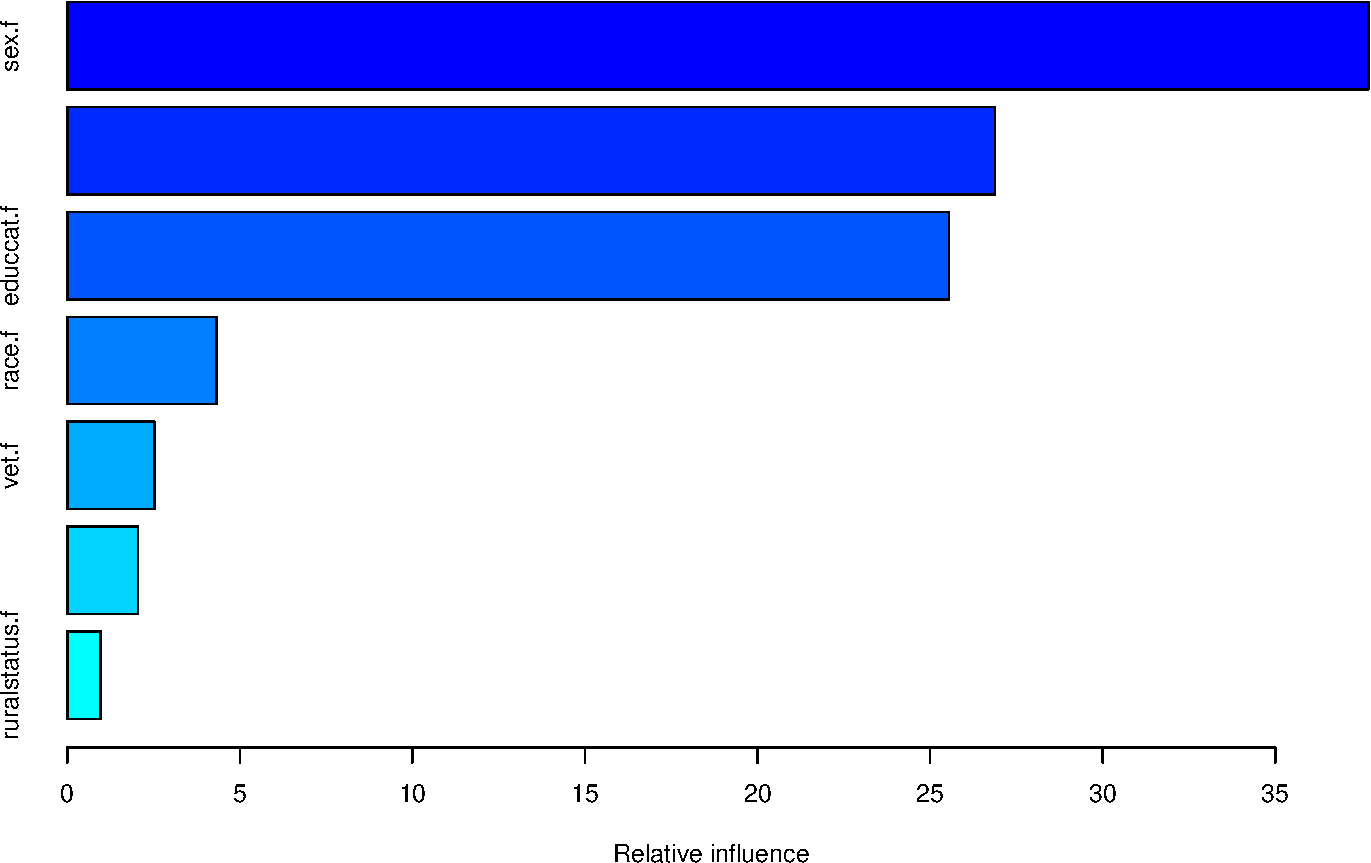
\includegraphics[keepaspectratio]{lab5_slides_files/figure-beamer/unnamed-chunk-6-1.pdf}}

\begin{verbatim}
##                         var    rel.inf
## sex.f                 sex.f 37.6952435
## married.f         married.f 26.8758977
## educcat.f         educcat.f 25.5532703
## race.f               race.f  4.3244764
## vet.f                 vet.f  2.5325575
## hispanic.f       hispanic.f  2.0532330
## ruralstatus.f ruralstatus.f  0.9653217
\end{verbatim}
\end{frame}

\begin{frame}[fragile]{Validating the Data}
\phantomsection\label{validating-the-data}
Now that we have trained the model, we want to look at how well it did.

We will first need to use \texttt{predict()} to generate the predicted
probabilities on the test dataset.

\scriptsize

\begin{Shaded}
\begin{Highlighting}[]
\NormalTok{morg\_test }\OtherTok{\textless{}{-}}\NormalTok{ morg\_test }\SpecialCharTok{|\textgreater{}}
  \FunctionTok{mutate}\NormalTok{(}\AttributeTok{pred =} \FunctionTok{predict}\NormalTok{(gbm1, }\AttributeTok{newdata =}\NormalTok{ morg\_test, }\AttributeTok{type =} \StringTok{"response"}\NormalTok{))}
\end{Highlighting}
\end{Shaded}

\begin{verbatim}
## Using 100 trees...
\end{verbatim}

\begin{Shaded}
\begin{Highlighting}[]
\FunctionTok{fivenum}\NormalTok{(morg\_test}\SpecialCharTok{$}\NormalTok{pred)}
\end{Highlighting}
\end{Shaded}

\begin{verbatim}
## [1] 0.001346357 0.009676978 0.019467815 0.035153008 0.111161584
\end{verbatim}
\end{frame}

\begin{frame}{Evaluating our model}
\phantomsection\label{evaluating-our-model}
Now that we have our predictions, we want to see how well we did

There are \textbf{many} different ways and metrics we can choose to do
this with

Which one is \emph{right} depends on the context of your problem (i.e.,
how costly are certain types of missclassifications)
\end{frame}

\begin{frame}{Confusion Matrix}
\phantomsection\label{confusion-matrix}
\begin{longtable}[]{@{}
  >{\raggedright\arraybackslash}p{(\linewidth - 4\tabcolsep) * \real{0.3333}}
  >{\raggedright\arraybackslash}p{(\linewidth - 4\tabcolsep) * \real{0.3333}}
  >{\raggedright\arraybackslash}p{(\linewidth - 4\tabcolsep) * \real{0.3333}}@{}}
\toprule\noalign{}
\begin{minipage}[b]{\linewidth}\raggedright
\end{minipage} & \begin{minipage}[b]{\linewidth}\raggedright
\textbf{Predicted Positive}
\end{minipage} & \begin{minipage}[b]{\linewidth}\raggedright
\textbf{Predicted Negative}
\end{minipage} \\
\midrule\noalign{}
\endhead
\textbf{Actual Positive} & TP & FN \\
\textbf{Actual Negative} & FP & TN \\
\bottomrule\noalign{}
\end{longtable}
\end{frame}

\begin{frame}{Precision and Recall}
\phantomsection\label{precision-and-recall}
\textbf{Precision}\\
Of all instances predicted \emph{positive}, the share that are truly
positive.\\
\[
\mathrm{Precision} = \frac{\mathrm{TP}}{\mathrm{TP} + \mathrm{FP}}
\]

\textbf{Recall (Sensitivity)}\\
Of all truly \emph{positive} instances, the share correctly
identified.\\
\[
\mathrm{Recall} = \frac{\mathrm{TP}}{\mathrm{TP} + \mathrm{FN}}
\]

\begin{itemize}
\tightlist
\item
  \textbf{High Precision} \(\Rightarrow\) Few false positives (when the
  model says ``yes,'' it's usually right).\\
\item
  \textbf{High Recall} \(\Rightarrow\) Few false negatives (the model
  finds most of the true positives).
\end{itemize}
\end{frame}

\begin{frame}{Threshold Selection}
\phantomsection\label{threshold-selection}
To turn a probability score into a class label, we choose a
\textbf{threshold} \(\tau\):

\[
  \hat y = 
  \begin{cases}
    1, & p \ge \tau,\\
    0, & p < \tau.
  \end{cases}
\]

\begin{itemize}
\tightlist
\item
  \textbf{Raising the threshold}

  \begin{itemize}
  \tightlist
  \item
    Fewer predicted positives \(\Rightarrow\) \textbf{Higher precision}
    \((\downarrow \mathrm{FP})\)\\
  \item
    More missed positives \(\Rightarrow\) \textbf{Lower recall}
    \((\uparrow \mathrm{FN})\)
  \end{itemize}
\item
  \textbf{Lowering the threshold}

  \begin{itemize}
  \tightlist
  \item
    More predicted positives \(\Rightarrow\) \textbf{Higher recall}
    \((\downarrow \mathrm{FN})\)\\
  \item
    More false alarms \(\Rightarrow\) \textbf{Lower precision}
    \((\uparrow \mathrm{FP})\)
  \end{itemize}
\item
  \textbf{Visualizing the trade‐off:}

  \begin{itemize}
  \tightlist
  \item
    \textbf{Precision--Recall curve:} plot precision vs.~recall as
    \(\tau\) varies.
  \end{itemize}
\end{itemize}
\end{frame}

\begin{frame}[fragile]{Calculating Metrics at the Default Threshold}
\phantomsection\label{calculating-metrics-at-the-default-threshold}
Let's compute recall and precision of our model at the default threshold
(0.50)

\tiny

\begin{Shaded}
\begin{Highlighting}[]
\NormalTok{morg\_test }\OtherTok{\textless{}{-}}\NormalTok{ morg\_test }\SpecialCharTok{|\textgreater{}}
  \FunctionTok{mutate}\NormalTok{(}\AttributeTok{class =} \FunctionTok{case\_when}\NormalTok{(pred }\SpecialCharTok{\textgreater{}} \FloatTok{0.5} \SpecialCharTok{\textasciitilde{}} \DecValTok{1}\NormalTok{,}
                           \ConstantTok{TRUE} \SpecialCharTok{\textasciitilde{}} \DecValTok{0}\NormalTok{))}

\NormalTok{confusion\_mat }\OtherTok{\textless{}{-}} \FunctionTok{count}\NormalTok{(morg\_test, class, mw)}

\NormalTok{tp }\OtherTok{\textless{}{-}}\NormalTok{ morg\_test }\SpecialCharTok{|\textgreater{}}
  \FunctionTok{filter}\NormalTok{(class }\SpecialCharTok{==} \DecValTok{1} \SpecialCharTok{\&}\NormalTok{ mw }\SpecialCharTok{==} \DecValTok{1}\NormalTok{) }\SpecialCharTok{|\textgreater{}}
  \FunctionTok{summarise}\NormalTok{(}\AttributeTok{tp =} \FunctionTok{n}\NormalTok{()) }\SpecialCharTok{\%\textgreater{}\%}
  \FunctionTok{pull}\NormalTok{(tp)}

\NormalTok{fn }\OtherTok{\textless{}{-}}\NormalTok{ morg\_test }\SpecialCharTok{|\textgreater{}}
  \FunctionTok{filter}\NormalTok{(class }\SpecialCharTok{==} \DecValTok{0} \SpecialCharTok{\&}\NormalTok{ mw }\SpecialCharTok{==} \DecValTok{1}\NormalTok{) }\SpecialCharTok{|\textgreater{}}
  \FunctionTok{summarise}\NormalTok{(}\AttributeTok{fn =} \FunctionTok{n}\NormalTok{()) }\SpecialCharTok{\%\textgreater{}\%}
  \FunctionTok{pull}\NormalTok{(fn)}

\NormalTok{fp }\OtherTok{\textless{}{-}}\NormalTok{ morg\_test }\SpecialCharTok{|\textgreater{}}
  \FunctionTok{filter}\NormalTok{(class }\SpecialCharTok{==} \DecValTok{1} \SpecialCharTok{\&}\NormalTok{ mw }\SpecialCharTok{==} \DecValTok{0}\NormalTok{) }\SpecialCharTok{|\textgreater{}}
  \FunctionTok{summarise}\NormalTok{(}\AttributeTok{fp =} \FunctionTok{n}\NormalTok{()) }\SpecialCharTok{\%\textgreater{}\%}
  \FunctionTok{pull}\NormalTok{(fp)}
\end{Highlighting}
\end{Shaded}
\end{frame}

\begin{frame}[fragile]{Calculating Metrics at the Default Threshold}
\phantomsection\label{calculating-metrics-at-the-default-threshold-1}
\scriptsize

\begin{Shaded}
\begin{Highlighting}[]
\NormalTok{recall }\OtherTok{\textless{}{-}}\NormalTok{ tp }\SpecialCharTok{/}\NormalTok{ (tp }\SpecialCharTok{+}\NormalTok{ fn)}

\NormalTok{percision }\OtherTok{\textless{}{-}}\NormalTok{ tp }\SpecialCharTok{/}\NormalTok{ (tp }\SpecialCharTok{+}\NormalTok{ fp)}

\NormalTok{recall}
\end{Highlighting}
\end{Shaded}

\begin{verbatim}
## [1] 0
\end{verbatim}

\begin{Shaded}
\begin{Highlighting}[]
\NormalTok{percision}
\end{Highlighting}
\end{Shaded}

\begin{verbatim}
## [1] NaN
\end{verbatim}
\end{frame}

\begin{frame}{Calculating Metrics at Many Thresholds}
\phantomsection\label{calculating-metrics-at-many-thresholds}
This will help us choose the value of recall and precision that provides
the best balance (or other criteria)

Let's compute these values for many different thresholds and plot the
\textbf{precision-recall curve}
\end{frame}

\begin{frame}[fragile]{Calculating Metrics at Many Thresholds}
\phantomsection\label{calculating-metrics-at-many-thresholds-1}
\tiny

\begin{Shaded}
\begin{Highlighting}[]
\NormalTok{pr\_curve\_tab }\OtherTok{\textless{}{-}} \FunctionTok{tibble}\NormalTok{()}

\ControlFlowTok{for}\NormalTok{ (i }\ControlFlowTok{in} \FunctionTok{seq}\NormalTok{(}\FloatTok{0.0001}\NormalTok{, }\FloatTok{0.9999}\NormalTok{, }\FloatTok{0.0001}\NormalTok{)) \{}
\NormalTok{  thresh }\OtherTok{\textless{}{-}}\NormalTok{ i}
\NormalTok{  morg\_test }\OtherTok{\textless{}{-}}\NormalTok{ morg\_test }\SpecialCharTok{|\textgreater{}}
    \FunctionTok{mutate}\NormalTok{(}\AttributeTok{class =} \FunctionTok{case\_when}\NormalTok{(pred }\SpecialCharTok{\textgreater{}}\NormalTok{ thresh }\SpecialCharTok{\textasciitilde{}} \DecValTok{1}\NormalTok{,}
                           \ConstantTok{TRUE} \SpecialCharTok{\textasciitilde{}} \DecValTok{0}\NormalTok{))}
\NormalTok{  tp }\OtherTok{\textless{}{-}}\NormalTok{ morg\_test }\SpecialCharTok{|\textgreater{}}
    \FunctionTok{filter}\NormalTok{(class }\SpecialCharTok{==} \DecValTok{1} \SpecialCharTok{\&}\NormalTok{ mw }\SpecialCharTok{==} \DecValTok{1}\NormalTok{) }\SpecialCharTok{|\textgreater{}}
    \FunctionTok{summarise}\NormalTok{(}\AttributeTok{tp =} \FunctionTok{n}\NormalTok{()) }\SpecialCharTok{\%\textgreater{}\%}
    \FunctionTok{pull}\NormalTok{(tp)}
\NormalTok{  fn }\OtherTok{\textless{}{-}}\NormalTok{ morg\_test }\SpecialCharTok{|\textgreater{}}
    \FunctionTok{filter}\NormalTok{(class }\SpecialCharTok{==} \DecValTok{0} \SpecialCharTok{\&}\NormalTok{ mw }\SpecialCharTok{==} \DecValTok{1}\NormalTok{) }\SpecialCharTok{|\textgreater{}}
    \FunctionTok{summarise}\NormalTok{(}\AttributeTok{fn =} \FunctionTok{n}\NormalTok{()) }\SpecialCharTok{\%\textgreater{}\%}
    \FunctionTok{pull}\NormalTok{(fn)}
\NormalTok{  fp }\OtherTok{\textless{}{-}}\NormalTok{ morg\_test }\SpecialCharTok{|\textgreater{}}
    \FunctionTok{filter}\NormalTok{(class }\SpecialCharTok{==} \DecValTok{1} \SpecialCharTok{\&}\NormalTok{ mw }\SpecialCharTok{==} \DecValTok{0}\NormalTok{) }\SpecialCharTok{|\textgreater{}}
    \FunctionTok{summarise}\NormalTok{(}\AttributeTok{fp =} \FunctionTok{n}\NormalTok{()) }\SpecialCharTok{\%\textgreater{}\%}
    \FunctionTok{pull}\NormalTok{(fp)}
\NormalTok{  recall }\OtherTok{\textless{}{-}}\NormalTok{ tp }\SpecialCharTok{/}\NormalTok{ (tp }\SpecialCharTok{+}\NormalTok{ fn)}
\NormalTok{  perc }\OtherTok{\textless{}{-}}\NormalTok{ tp }\SpecialCharTok{/}\NormalTok{ (tp }\SpecialCharTok{+}\NormalTok{ fp)}
\NormalTok{  tab }\OtherTok{\textless{}{-}} \FunctionTok{tibble}\NormalTok{(thresh, recall, perc)}
\NormalTok{  pr\_curve\_tab }\OtherTok{\textless{}{-}} \FunctionTok{bind\_rows}\NormalTok{(pr\_curve\_tab, tab)}
\NormalTok{\}}
\end{Highlighting}
\end{Shaded}
\end{frame}

\begin{frame}[fragile]{Plotting the PR Curve}
\phantomsection\label{plotting-the-pr-curve}
\tiny

\begin{Shaded}
\begin{Highlighting}[]
\DocumentationTok{\#\# Print curve}

\NormalTok{p1 }\OtherTok{\textless{}{-}} \FunctionTok{ggplot}\NormalTok{(pr\_curve\_tab) }\SpecialCharTok{+}
  \FunctionTok{geom\_path}\NormalTok{(}\FunctionTok{aes}\NormalTok{(}\AttributeTok{x =}\NormalTok{ recall, }\AttributeTok{y =}\NormalTok{ perc)) }\SpecialCharTok{+}
  \FunctionTok{coord\_cartesian}\NormalTok{(}\AttributeTok{ylim =} \FunctionTok{c}\NormalTok{(}\DecValTok{0}\NormalTok{, }\FloatTok{0.25}\NormalTok{))}

\FunctionTok{print}\NormalTok{(p1)}
\end{Highlighting}
\end{Shaded}

\begin{verbatim}
## Warning: Removed 8888 rows containing missing values or values outside the scale range
## (`geom_path()`).
\end{verbatim}

\pandocbounded{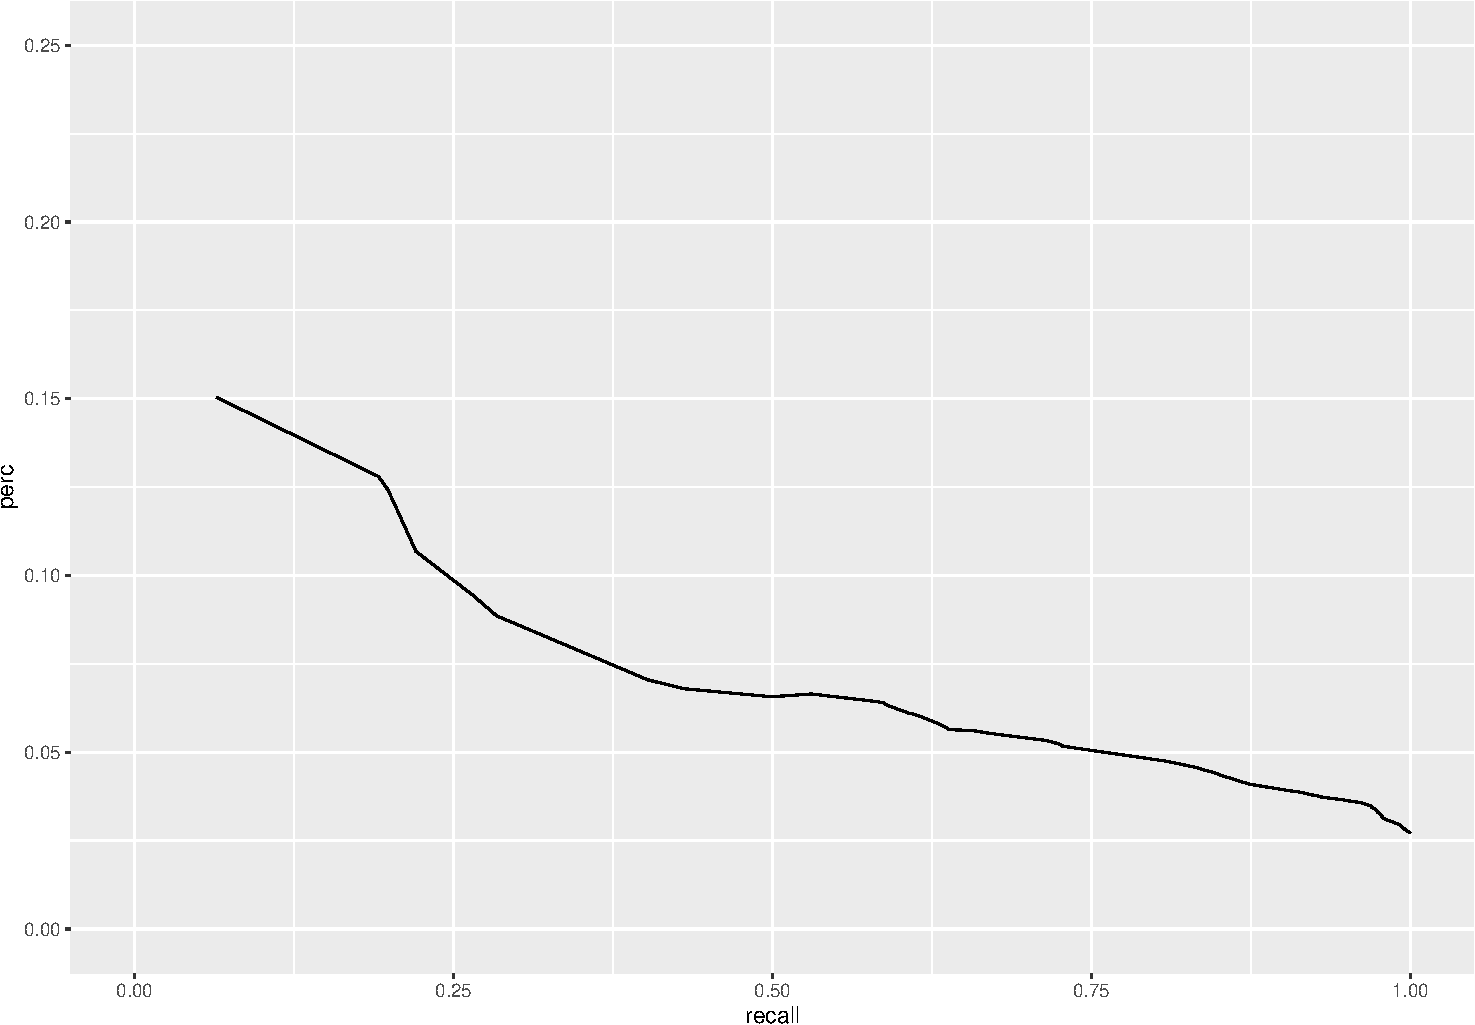
\includegraphics[keepaspectratio]{lab5_slides_files/figure-beamer/unnamed-chunk-11-1.pdf}}
\end{frame}

\begin{frame}[fragile]{The High-Recall Group}
\phantomsection\label{the-high-recall-group}
Let's say that we want to optimize the recall rate to be about 75\%

Let's find the point on our curve where this holds and the associated
threshold value

\scriptsize

\begin{Shaded}
\begin{Highlighting}[]
\NormalTok{pr\_curve\_tab }\SpecialCharTok{\%\textgreater{}\%}
  \FunctionTok{filter}\NormalTok{(recall }\SpecialCharTok{\textgreater{}} \FloatTok{0.74} \SpecialCharTok{\&}\NormalTok{ recall }\SpecialCharTok{\textless{}} \FloatTok{0.76}\NormalTok{)}
\end{Highlighting}
\end{Shaded}

\begin{verbatim}
## # A tibble: 0 x 3
## # i 3 variables: thresh <dbl>, recall <dbl>, perc <dbl>
\end{verbatim}

\begin{Shaded}
\begin{Highlighting}[]
\NormalTok{final\_threshold }\OtherTok{\textless{}{-}} \FloatTok{0.025}
\end{Highlighting}
\end{Shaded}
\end{frame}

\begin{frame}[fragile]{Predicting the outcome for the full data}
\phantomsection\label{predicting-the-outcome-for-the-full-data}
Now that we have trained our model and chosen the appropriate threshold,
we can finally generate the predicted values for our full dataset

\scriptsize

\begin{Shaded}
\begin{Highlighting}[]
\NormalTok{morg }\OtherTok{\textless{}{-}}\NormalTok{ morg }\SpecialCharTok{|\textgreater{}}
  \FunctionTok{mutate}\NormalTok{(}\AttributeTok{pred\_class =} \FunctionTok{predict}\NormalTok{(gbm1, }\AttributeTok{newdata =}\NormalTok{ morg, }\AttributeTok{type =} \StringTok{"response"}\NormalTok{))}
\end{Highlighting}
\end{Shaded}

\begin{verbatim}
## Using 100 trees...
\end{verbatim}

\begin{Shaded}
\begin{Highlighting}[]
\NormalTok{morg }\OtherTok{\textless{}{-}}\NormalTok{ morg }\SpecialCharTok{|\textgreater{}}
  \FunctionTok{mutate}\NormalTok{(}\AttributeTok{pred\_mw =} \FunctionTok{case\_when}\NormalTok{(pred\_class }\SpecialCharTok{\textgreater{}}\NormalTok{ final\_threshold }\SpecialCharTok{\textasciitilde{}} \DecValTok{1}\NormalTok{,}
                             \FunctionTok{is.na}\NormalTok{(pred\_class) }\SpecialCharTok{\textasciitilde{}} \ConstantTok{NA\_real\_}\NormalTok{,}
                             \ConstantTok{TRUE} \SpecialCharTok{\textasciitilde{}} \DecValTok{0}\NormalTok{))}
\NormalTok{morg }\SpecialCharTok{|\textgreater{}}
  \FunctionTok{group\_by}\NormalTok{(pred\_mw) }\SpecialCharTok{|\textgreater{}}
  \FunctionTok{summarise}\NormalTok{(}\AttributeTok{n =} \FunctionTok{n}\NormalTok{(),}
            \AttributeTok{mean\_wage =} \FunctionTok{mean}\NormalTok{(earnhre, }\AttributeTok{na.rm =}\NormalTok{ T))}
\end{Highlighting}
\end{Shaded}

\begin{verbatim}
## # A tibble: 2 x 3
##   pred_mw       n mean_wage
##     <dbl>   <int>     <dbl>
## 1       0 2740097      772.
## 2       1 1386779      519.
\end{verbatim}
\end{frame}

\end{document}
